%\begin{enumerate}[label=\thesubsection.\arabic*.,ref=\thesubsection.\theenumi]
%\numberwithin{equation}{enumi}

%\item 
Obtain the transfer function from the frequency response data given below.
\begin{table}[!ht]
\centering
\begin{enumerate}[label=\thesection.\arabic*.,ref=\thesection.\theenumi]
\numberwithin{equation}{enumi}
\item State the general model of a state space system specifying the dimensions of the matrices and vectors.
\\
\solution The model is given by 
\begin{align}
\dot{\vec{x}}(t)&=\vec{A}\vec{x}(t)+\vec{B}\vec{u}(t) \\
 \vec{y}(t)&=\vec{C}\vec{x}(t)+\vec{D} \vec{u}(t)
\end{align}
with parameters listed in Table \ref{table:ee18btech11004}.
%
\begin{table}[!ht]
\centering
\begin{enumerate}[label=\thesubsection.\arabic*.,ref=\thesubsection.\theenumi]
\numberwithin{equation}{enumi}
\item State the general model of a state space system specifying the dimensions of the matrices and vectors.
\\
\solution The model is given by 
\begin{align}
\label{eq:ee18btech11004_state}
\dot{\vec{x}}(t)&=\vec{A}\vec{x}(t)+\vec{B}\vec{u}(t) \\
 \vec{y}(t)&=\vec{C}\vec{x}(t)+\vec{D} \vec{u}(t)
\end{align}
%
with parameters listed in Table \ref{table:ee18btech11004}.
%
\begin{table}[!ht]
\centering
\begin{enumerate}[label=\thesubsection.\arabic*.,ref=\thesubsection.\theenumi]
\numberwithin{equation}{enumi}
\item State the general model of a state space system specifying the dimensions of the matrices and vectors.
\\
\solution The model is given by 
\begin{align}
\label{eq:ee18btech11004_state}
\dot{\vec{x}}(t)&=\vec{A}\vec{x}(t)+\vec{B}\vec{u}(t) \\
 \vec{y}(t)&=\vec{C}\vec{x}(t)+\vec{D} \vec{u}(t)
\end{align}
%
with parameters listed in Table \ref{table:ee18btech11004}.
%
\begin{table}[!ht]
\centering
\input{./tables/ee18btech11004.tex}
\caption{}
\label{table:ee18btech11004}
\end{table}
\item Find the transfer function $\vec{H}(s)$ for the general system.
\\
\solution 
Taking Laplace transform on both sides we have the following equations
\begin{align}
 s\vec{IX}(s)-\vec{x}(0)&= \vec{AX}(s)+ \vec{BU}(s)\\
(s\vec{I}-\vec{A})\vec{X}(s)&= \vec{BU}(s)+ \vec{x}(0)\\
\vec{X}(s)&={(s\vec{I}-\vec{A})^{-1}}\vec{B U}(s)\\
& +(s\vec{I}-\vec{A})^{-1}\vec{x}(0)
\label{eq:x_init}
\end{align}
and
\begin{align}
\vec{Y}(s)&= \vec{CX}(s)+D\vec{IU}(s)
\end{align}
Substituting from \eqref{eq:x_init} in the above,
%
\begin{multline}
\vec{Y}(s)=( \vec{C}{(s\vec{I}-\vec{A})^{-1}}\vec{B}+D\vec{I}) \vec{U}(s) 
\\
+ \vec{C}(s\vec{I}-\vec{A})^{-1}\vec{x}(0)
\end{multline}
%
%
\item Find $H(s)$ for a SISO (single input single output) system.
\\
\solution
\begin{align}
\label{eq:ee18btech11004_siso}
H(s)= {\frac{Y(s)}{U(s)}}= C{(sI-A)^{-1}}B+DI
\end{align}

\item Given 
\begin{align}
H(s)&=\frac{1}{s^3+3s^2+2s+1}
\\
D&=0
\\
\vec{B}&= \myvec{0\\0\\1}
\end{align}
%
 find $\vec{A}$ and $\vec{C}$ such that the state-space realization is in {\em controllable canonical form}.
\\
\solution 
\begin{align} 
\because {\frac{Y(s)}{U(s)}}= \frac{Y(s)}{V(s)} \times \frac{V(s)}{U(s)},
\end{align}
letting
\begin{align}
 {\frac{Y(s)}{V(s)}}= 1, 
\end{align}
results in 
\begin{align}
{\frac{U(s)}{V(s)}}={s^3 + 3s^2+2s + 1}
\end{align}

giving
\begin{align}
U(s)= s^3 V(s) + 3s^2 V(s)+2sV(s) + V(s)
\end{align}

so equation 0.1.13 can be written as
\begin{align}
\myvec{sV(s)\\s^2V(s)\\s^3V(s)}
=
\myvec{0&1&0\\0&0&1\\-1&-2&-3}\myvec{V(s)\\s(s)\\s^2V(s)}
+
\myvec{0\\0\\1}  U
\end{align}
So 
\begin{align}
\vec{A}=\myvec{0&1&0\\0&0&1\\-1&-2&-3}
\end{align}

\begin{align}
Y=X_{1}(s)
=\myvec{1&0&0} \myvec{V(s)\\sV(s)\\s^2V(s)}
\end{align}
\begin{align}
\vec{C}=\myvec{1&0&0}
\end{align}

\item Obtain $\vec{A}$ and $\vec{C}$ so that the state-space realization in in {\em observable canonical form}.
\\
\solution  Given that
\begin{align}
H(s)&=\frac{1}{s^3+3s^2+2s+1}
\end{align}
\begin{align}
\frac{Y(s)}{U(s)}=\frac{1}{s^3+3s^2+2s+1} \\
Y(s) \times (s^3+3s^2+2s+1) = U(s)
\end{align}
\begin{align}
s^3Y(s)+3s^2Y(s)+2sY(s)+Y(s)=U(s)\\
s^3Y(s)=U(s)-3s^2Y(s)-2sY(s)-Y(s)\\
Y(s)=-3s^{-1}Y(s)-2s^{-2}Y(s)+s^{-3}(U(s)-Y(s))
\end{align}
\\ let $Y=aU+X_{1}$
\\ by comparing with equation 1.5.6 we get a=0 and
\begin{align}
Y=X_{1}
\end{align}
inverse laplace transform of above equation is 
\begin{align}
y=x_{1}
\end{align}
so from above equation 1.5.6 and 1.5.7
\begin{align}
X_{1}=-3s^{-1}Y(s)-2s^{-2}Y(s)+s^{-3}(U(s)-Y(s))\\
sX_{1}=-3Y(s)-2s^{-1}Y(s)+s^{-2}(U(s)-Y(s)) 
\end{align}
inverse laplace transform of above equation 
\begin{align}
\dot{x_{1}}=-3y+x_{2}
\end{align} 
where
\begin{align}
X_{2}=-2s^{-1}Y(s)+s^{-2}(U(s)-Y(s))\\
sX_{2}=-2Y(s)+s^{-1}(U(s)-Y(s))
\end{align} 
inverse laplace transform of above equation 
\begin{align}
\dot{x_{2}}=-2y+x_{3}
\end{align}
where
\begin{align}
X_{3}=s^{-1}(U(s)-Y(s))\\
sX_{3}=U(s)-Y(s)
\end{align} 
inverse laplace transform of above equation 
\begin{align}
\dot{x_{3}}=u-y
\end{align}
so we get four equations which are
\begin{align}
y=x_{1}\\
\dot{x_{1}}=-3y+x_{2}\\
\dot{x_{2}}=-2y+x_{3}\\
\dot{x_{3}}=u-y
\end{align} 
sub $ y=x_{1}$ in 1.5.19,1.5.20,1.5.21 we get
\begin{align}
 y=x_{1}\\
\dot{x_{1}}=-3x_{1}+x_{2}\\
\dot{x_{2}}=-2x_{1}+x_{3}\\
\dot{x_{3}}=u-x_{1}
\end{align} 
so above equations can be written as
\begin{align}
\myvec{\dot{x_{1}}\\\dot{x_{2}}\\\dot{x_{3}})}
=
\myvec{-3&1&0\\-2&0&1\\-1&0&0}\myvec{x_{1}\\x_{2}\\x_{3}}
+
\myvec{0\\0\\1}  U
\end{align}
So 
\begin{align}
\vec{A}=\myvec{-3&1&0\\-2&0&1\\-1&0&0}
\end{align}
\begin{align}
y=x_{1}
=\myvec{1&0&0} \myvec{x_{1}\\x_{2}\\x_{3}}
\end{align}
\begin{align}
\vec{C}=\myvec{1&0&0}
\end{align}


\item Find the eigenvaues of $\vec{A}$ and the poles of $H(s)$ using a python code.
\\
\solution The following code 
%
\begin{lstlisting}
codes/ee18btech11004.py
\end{lstlisting}
gives the necessary values.  The roots are the same as the eigenvalues.
%
\item Theoretically, show that eigenvaues of $\vec{A}$ are the poles of  $H(s)$.
\solution 
\\ as we know tthat  the characteristic equation is det(sI-A) 
\\\begin{align}
\vec{sI-A}=
\myvec{s&0&0\\0&s&0\\0&0&s}
-
\myvec{0&1&0\\0&0&1\\-1&-2&-3}
=\myvec{s&-1&0\\0&s&-1\\1&2&s+3}
\end{align}
\\therfore
\begin{align}
det(sI-A)=s(s^2+3s+2)+1(1)=s^3+3s^2+2s+1
\end{align} 
\\so from equation 1.6.2 we can see that charcteristic equation is equal to the denominator of the transefer function
\end{enumerate}


\caption{}
\label{table:ee18btech11004}
\end{table}
\item Find the transfer function $\vec{H}(s)$ for the general system.
\\
\solution 
Taking Laplace transform on both sides we have the following equations
\begin{align}
 s\vec{IX}(s)-\vec{x}(0)&= \vec{AX}(s)+ \vec{BU}(s)\\
(s\vec{I}-\vec{A})\vec{X}(s)&= \vec{BU}(s)+ \vec{x}(0)\\
\vec{X}(s)&={(s\vec{I}-\vec{A})^{-1}}\vec{B U}(s)\\
& +(s\vec{I}-\vec{A})^{-1}\vec{x}(0)
\label{eq:x_init}
\end{align}
and
\begin{align}
\vec{Y}(s)&= \vec{CX}(s)+D\vec{IU}(s)
\end{align}
Substituting from \eqref{eq:x_init} in the above,
%
\begin{multline}
\vec{Y}(s)=( \vec{C}{(s\vec{I}-\vec{A})^{-1}}\vec{B}+D\vec{I}) \vec{U}(s) 
\\
+ \vec{C}(s\vec{I}-\vec{A})^{-1}\vec{x}(0)
\end{multline}
%
%
\item Find $H(s)$ for a SISO (single input single output) system.
\\
\solution
\begin{align}
\label{eq:ee18btech11004_siso}
H(s)= {\frac{Y(s)}{U(s)}}= C{(sI-A)^{-1}}B+DI
\end{align}

\item Given 
\begin{align}
H(s)&=\frac{1}{s^3+3s^2+2s+1}
\\
D&=0
\\
\vec{B}&= \myvec{0\\0\\1}
\end{align}
%
 find $\vec{A}$ and $\vec{C}$ such that the state-space realization is in {\em controllable canonical form}.
\\
\solution 
\begin{align} 
\because {\frac{Y(s)}{U(s)}}= \frac{Y(s)}{V(s)} \times \frac{V(s)}{U(s)},
\end{align}
letting
\begin{align}
 {\frac{Y(s)}{V(s)}}= 1, 
\end{align}
results in 
\begin{align}
{\frac{U(s)}{V(s)}}={s^3 + 3s^2+2s + 1}
\end{align}

giving
\begin{align}
U(s)= s^3 V(s) + 3s^2 V(s)+2sV(s) + V(s)
\end{align}

so equation 0.1.13 can be written as
\begin{align}
\myvec{sV(s)\\s^2V(s)\\s^3V(s)}
=
\myvec{0&1&0\\0&0&1\\-1&-2&-3}\myvec{V(s)\\s(s)\\s^2V(s)}
+
\myvec{0\\0\\1}  U
\end{align}
So 
\begin{align}
\vec{A}=\myvec{0&1&0\\0&0&1\\-1&-2&-3}
\end{align}

\begin{align}
Y=X_{1}(s)
=\myvec{1&0&0} \myvec{V(s)\\sV(s)\\s^2V(s)}
\end{align}
\begin{align}
\vec{C}=\myvec{1&0&0}
\end{align}

\item Obtain $\vec{A}$ and $\vec{C}$ so that the state-space realization in in {\em observable canonical form}.
\\
\solution  Given that
\begin{align}
H(s)&=\frac{1}{s^3+3s^2+2s+1}
\end{align}
\begin{align}
\frac{Y(s)}{U(s)}=\frac{1}{s^3+3s^2+2s+1} \\
Y(s) \times (s^3+3s^2+2s+1) = U(s)
\end{align}
\begin{align}
s^3Y(s)+3s^2Y(s)+2sY(s)+Y(s)=U(s)\\
s^3Y(s)=U(s)-3s^2Y(s)-2sY(s)-Y(s)\\
Y(s)=-3s^{-1}Y(s)-2s^{-2}Y(s)+s^{-3}(U(s)-Y(s))
\end{align}
\\ let $Y=aU+X_{1}$
\\ by comparing with equation 1.5.6 we get a=0 and
\begin{align}
Y=X_{1}
\end{align}
inverse laplace transform of above equation is 
\begin{align}
y=x_{1}
\end{align}
so from above equation 1.5.6 and 1.5.7
\begin{align}
X_{1}=-3s^{-1}Y(s)-2s^{-2}Y(s)+s^{-3}(U(s)-Y(s))\\
sX_{1}=-3Y(s)-2s^{-1}Y(s)+s^{-2}(U(s)-Y(s)) 
\end{align}
inverse laplace transform of above equation 
\begin{align}
\dot{x_{1}}=-3y+x_{2}
\end{align} 
where
\begin{align}
X_{2}=-2s^{-1}Y(s)+s^{-2}(U(s)-Y(s))\\
sX_{2}=-2Y(s)+s^{-1}(U(s)-Y(s))
\end{align} 
inverse laplace transform of above equation 
\begin{align}
\dot{x_{2}}=-2y+x_{3}
\end{align}
where
\begin{align}
X_{3}=s^{-1}(U(s)-Y(s))\\
sX_{3}=U(s)-Y(s)
\end{align} 
inverse laplace transform of above equation 
\begin{align}
\dot{x_{3}}=u-y
\end{align}
so we get four equations which are
\begin{align}
y=x_{1}\\
\dot{x_{1}}=-3y+x_{2}\\
\dot{x_{2}}=-2y+x_{3}\\
\dot{x_{3}}=u-y
\end{align} 
sub $ y=x_{1}$ in 1.5.19,1.5.20,1.5.21 we get
\begin{align}
 y=x_{1}\\
\dot{x_{1}}=-3x_{1}+x_{2}\\
\dot{x_{2}}=-2x_{1}+x_{3}\\
\dot{x_{3}}=u-x_{1}
\end{align} 
so above equations can be written as
\begin{align}
\myvec{\dot{x_{1}}\\\dot{x_{2}}\\\dot{x_{3}})}
=
\myvec{-3&1&0\\-2&0&1\\-1&0&0}\myvec{x_{1}\\x_{2}\\x_{3}}
+
\myvec{0\\0\\1}  U
\end{align}
So 
\begin{align}
\vec{A}=\myvec{-3&1&0\\-2&0&1\\-1&0&0}
\end{align}
\begin{align}
y=x_{1}
=\myvec{1&0&0} \myvec{x_{1}\\x_{2}\\x_{3}}
\end{align}
\begin{align}
\vec{C}=\myvec{1&0&0}
\end{align}


\item Find the eigenvaues of $\vec{A}$ and the poles of $H(s)$ using a python code.
\\
\solution The following code 
%
\begin{lstlisting}
codes/ee18btech11004.py
\end{lstlisting}
gives the necessary values.  The roots are the same as the eigenvalues.
%
\item Theoretically, show that eigenvaues of $\vec{A}$ are the poles of  $H(s)$.
\solution 
\\ as we know tthat  the characteristic equation is det(sI-A) 
\\\begin{align}
\vec{sI-A}=
\myvec{s&0&0\\0&s&0\\0&0&s}
-
\myvec{0&1&0\\0&0&1\\-1&-2&-3}
=\myvec{s&-1&0\\0&s&-1\\1&2&s+3}
\end{align}
\\therfore
\begin{align}
det(sI-A)=s(s^2+3s+2)+1(1)=s^3+3s^2+2s+1
\end{align} 
\\so from equation 1.6.2 we can see that charcteristic equation is equal to the denominator of the transefer function
\end{enumerate}


\caption{}
\label{table:ee18btech11004}
\end{table}

\item Find the transfer function $\vec{H}(s)$ for the general system.
\\
\solution 
Taking Laplace transform on both sides we have the following equations
\begin{align}
 s\vec{IX}(s)-\vec{x}(0)&= \vec{AX}(s)+ \vec{BU}(s)\\
(s\vec{I}-\vec{A})\vec{X}(s)&= \vec{BU}(s)+ \vec{x}(0)\\
\vec{X}(s)&={(s\vec{I}-\vec{A})^{-1}}\vec{B U}(s)\\
& +(s\vec{I}-\vec{A})^{-1}\vec{x}(0)
\label{eq:x_init}
\end{align}
and
\begin{align}
\vec{Y}(s)&= \vec{CX}(s)+D\vec{IU}(s)
\end{align}
Substituting from \eqref{eq:x_init} in the above,
%
\begin{multline}
\vec{Y}(s)=( \vec{C}{(s\vec{I}-\vec{A})^{-1}}\vec{B}+D\vec{I}) \vec{U}(s) 
\\
+ \vec{C}(s\vec{I}-\vec{A})^{-1}\vec{x}(0)
\end{multline}
%
\item Find $H(s)$ for a SISO (single input single output) system.
\\
\solution
\begin{align}
\label{eq:ee18btech11004_siso}
H(s)= {\frac{Y(s)}{U(s)}}= \vec{C}{(s\vec{I}-\vec{A})^{-1}}\vec{B}+D\vec{I}
\end{align}

\item Given 
\begin{align}
\label{eq:ee18btech11004_system}
H(s)&=\frac{1}{s^3+3s^2+2s+1}
\\
D&=0
\\
\vec{B}&= \myvec{0\\0\\1}
\end{align}
%
 find $\vec{A}$ and $\vec{C}$ such that the state-space realization is in {\em controllable canonical form}.
\\
\solution 
\begin{align} 
\because {\frac{Y(s)}{U(s)}}= \frac{Y(s)}{V(s)} \times \frac{V(s)}{U(s)},
\end{align}
letting
\begin{align}
 {\frac{Y(s)}{V(s)}}= 1, 
\end{align}
results in 
\begin{align}
{\frac{U(s)}{V(s)}}={s^3 + 3s^2+2s + 1}
\end{align}

giving
\begin{align}
U(s)= s^3 V(s) + 3s^2 V(s)+2sV(s) + V(s)
\end{align}
%
so the above equation  can be written as
\begin{align}
\myvec{sV(s)\\s^2V(s)\\s^3V(s)}
=
\myvec{0&1&0\\0&0&1\\-1&-2&-3}\myvec{V(s)\\sV(s)\\s^2V(s)}
+
\myvec{0\\0\\1}  U
\end{align}
Letting
\begin{align}
\vec{A}&=\myvec{0&1&0\\0&0&1\\-1&-2&-3}
\\
\vec{X}_1 &= \myvec{sV(s)\\s^2V(s)\\s^3V(s)}
\\
\vec{X} &= \myvec{V(s)\\sV(s)\\s^2V(s)},
\end{align}
\\
\begin{align}
\vec{X}_{1}(s) &= \vec{A}\vec{X}(s)+ \vec{B}U(s)
\\
Y&=\vec{C}\vec{X}_{1}(s)
\end{align}
where
\begin{align}
\vec{C}=\myvec{1&0&0}
\end{align}

\item Obtain $\vec{A}$ and $\vec{C}$ so that the state-space realization in in {\em observable canonical form}.
\\
\solution  Given that
\begin{align}
H(s)&=\frac{1}{s^3+3s^2+2s+1},
\\
%\end{align}
%\begin{align}
\frac{Y(s)}{U(s)}&=\frac{1}{s^3+3s^2+2s+1} \\
\implies  U(s)&=Y(s)  (s^3+3s^2+2s+1)
%\end{align}
%\begin{align}
%U(s)&=s^3Y(s)+3s^2Y(s)+2sY(s)+Y(s)\\
%s^3Y(s)&=U(s)-3s^2Y(s)-2sY(s)-Y(s)\\
\\
\text{or, }Y(s)&=-3s^{-1}Y(s)-2s^{-2}Y(s)+
\nonumber \\
&\quad s^{-3}(U(s)-Y(s))
\end{align}
%\\ let $Y=aU+X_{1}$
%\\ by comparing with equation 1.5.6 we get a=0 and
%so from above equation 1.5.6 and 1.5.7
Let
\begin{align}
X_{1}(s)&=Y(s) = -3s^{-1}Y(s)-2s^{-2}Y(s) \nonumber \\
&\quad +s^{-3}(U(s)-Y(s))\\
%sX_{1}(s)&=-3Y(s)-2s^{-1}Y(s)\\ 
%&+s^{-2}(U(s)-Y(s))
%\end{align} 
%\begin{align}
%sX_{1}(s)&=-3Y(s)+X_{2}(s)
%\end{align} 
%where
%\begin{align}
X_{2}(s)&=-2s^{-1}Y(s)+s^{-2}(U(s)-Y(s))\\
%sX_{2}(s)&=-2Y(s)+s^{-1}(U(s)-Y(s))
%\end{align} 
%\begin{align}
%sX_{2}(s)&=-2Y(s)+X_{3}(s)
%\end{align}
%where
%\begin{align}
X_{3}(s)&=s^{-1}(U(s)-Y(s))
%sX_{3}(s)&=U(s)-Y(s)
\end{align} 
%\begin{align}
%X_{3}(s)&=U(s)-Y(s)
%\end{align}
\begin{align}
\implies
\begin{split}
sX_{1}(s)&=-3Y(s)+X_{2}(s)\\
sX_{2}(s)&=-2Y(s)+X_{3}(s)\\
sX_{3}(s)&=U(s)-Y(s)
\end{split}
\end{align} 
Substituting  $ Y=X_{1}(s)$ the above, 
\begin{align}
sX_{1}(s)&=-3X_{1}(s)+X_{2}(s)\\
sX_{2}(s)&=-2X_{1}(s)+X_{3}(s)\\
sX_{3}(s)&=U(s)-X_{1}(s)
\end{align} 
which can be expressed as
\begin{align}
\myvec{sX_{1}(s)\\sX_{2}(s)\\sX_{3}(s)}
&=
\myvec{-3&1&0\\-2&0&1\\-1&0&0}\myvec{X_{1}(s)\\X_{2}(s)\\X_{3}(s)}
+
\myvec{0\\0\\1}  U
\\
\text{or, }
\begin{split}
s\vec{X}(s) &= \vec{A}\vec{X}(s) + \vec{B}U(s)
\\
Y(s) &= \vec{B}\vec{X}(s)
\end{split}
\end{align}
where
\begin{align}
\vec{A}&=\myvec{-3&1&0\\-2&0&1\\-1&0&0}
\\
\vec{B}&= \myvec{1&0&0}
\end{align}
%\begin{align}
%Y(s)=X_{1}(s)
%=\myvec{1&0&0} \myvec{X_{1}(s)\\X_{2}(s)\\X_{3}(s)}
%\end{align}
%\begin{align}
%\vec{C}&=\myvec{1&0&0}
%\end{align}
%
%
%
%\\
%\solution  Given that
%\begin{align}
%H(s)&=\frac{1}{s^3+3s^2+2s+1},
%\\
%\frac{Y(s)}{U(s)}&=\frac{1}{s^3+3s^2+2s+1} \\
%%\implies  U(s)&= (s^3+3s^2+2s+1)Y(s) 
%%\\
%%\implies 
%%U(s)&=s^3Y(s)+3s^2Y(s)+2sY(s)+Y(s)\\
%%s^3Y(s)&=U(s)-3s^2Y(s)-2sY(s)-Y(s)\\
%\implies Y(s)&=-3s^{-1}Y(s)-2s^{-2}Y(s) \nonumber \\
%&\quad +s^{-3}\brak{U(s)-Y(s)}
%\end{align}
%%
%after some algebra.
%\\ let $Y=aU+X_{1}$
%\\ by comparing with equation 1.5.6 we get a=0 and
%\begin{align}
%Y=X_{1}
%\end{align}
%inverse laplace transform of above equation is 
%\begin{align}
%y=x_{1}
%\end{align}
%so from above equation 1.5.6 and 1.5.7
%\begin{align}
%X_{1}&=-3s^{-1}Y(s)-2s^{-2}Y(s)+s^{-3}(U(s)-Y(s))\\
%sX_{1}&=-3Y(s)-2s^{-1}Y(s)+s^{-2}(U(s)-Y(s)) 
%\end{align}
%inverse laplace transform of above equation 
%\begin{align}
%\dot{x_{1}}&=-3y+x_{2}
%\end{align} 
%where
%\begin{align}
%X_{2}&=-2s^{-1}Y(s)+s^{-2}(U(s)-Y(s))\\
%sX_{2}&=-2Y(s)+s^{-1}(U(s)-Y(s))
%\end{align} 
%inverse laplace transform of above equation 
%\begin{align}
%\dot{x_{2}}&=-2y+x_{3}
%\end{align}
%where
%\begin{align}
%X_{3}&=s^{-1}(U(s)-Y(s))\\
%sX_{3}&=U(s)-Y(s)
%\end{align} 
%inverse laplace transform of above equation 
%\begin{align}
%\dot{x_{3}}&=u-y
%\end{align}
%so we get four equations which are
%\begin{align}
%x_{1}&=y\\
%\dot{x_{1}}&=-3y+x_{2}\\
%\dot{x_{2}}&=-2y+x_{3}\\
%\dot{x_{3}}&=u-y
%\end{align} 
%sub $ y=x_{1}$ in 1.5.19,1.5.20,1.5.21 we get
%\begin{align}
%x_{1}&=y\\
%\dot{x_{1}}&=-3x_{1}+x_{2}\\
%\dot{x_{2}}&=-2x_{1}+x_{3}\\
%\dot{x_{3}}&=u-x_{1}
%\end{align} 
%so above equations can be written as
%\begin{align}
%\myvec{\dot{x_{1}}\\\dot{x_{2}}\\\dot{x_{3}})}
%=
%\myvec{-3&1&0\\-2&0&1\\-1&0&0}\myvec{x_{1}\\x_{2}\\x_{3}}
%+
%\myvec{0\\0\\1}  U
%\end{align}
%So 
%\begin{align}
%\vec{A}=\myvec{-3&1&0\\-2&0&1\\-1&0&0}
%\end{align}
%\begin{align}
%y=x_{1}
%=\myvec{1&0&0} \myvec{x_{1}\\x_{2}\\x_{3}}
%\end{align}
%\begin{align}
%\vec{C}&=\myvec{1&0&0}
%\end{align}
%

\item Find the eigenvaues of $\vec{A}$ and the poles of $H(s)$ using a python code.
\\
\solution The following code 
%
\begin{lstlisting}
codes/ee18btech11004.py
\end{lstlisting}
gives the necessary values.  The roots are the same as the eigenvalues.
%
\item Theoretically, show that eigenvaues of $\vec{A}$ are the poles of  $H(s)$.\\
\solution 
As we know that  the characteristic equation is det(sI-A) 
\\\begin{align}
s\vec{I}-\vec{A}=
\myvec{s&0&0\\0&s&0\\0&0&s}
-
\myvec{0&1&0\\0&0&1\\-1&-2&-3}\\
=\myvec{s&-1&0\\0&s&-1\\1&2&s+3}
\end{align}

\begin{align}
\implies \mydet{s\vec{I}-\vec{A}}&=s(s^2+3s+2)+1(1)\\
&=s^3+3s^2+2s+1
\end{align} 
which is the denominator of $H(s)$ in \eqref{eq:ee18btech11004_system}
%
\end{enumerate}


\caption{}
\label{table:ee18btech11006}
\end{table}
\solution 
The following code generates the plot for the given data.
\begin{lstlisting}
codes/ee18btech11006/ee18btech11006_1.py
\end{lstlisting}
\begin{figure}[!ht]
\centering
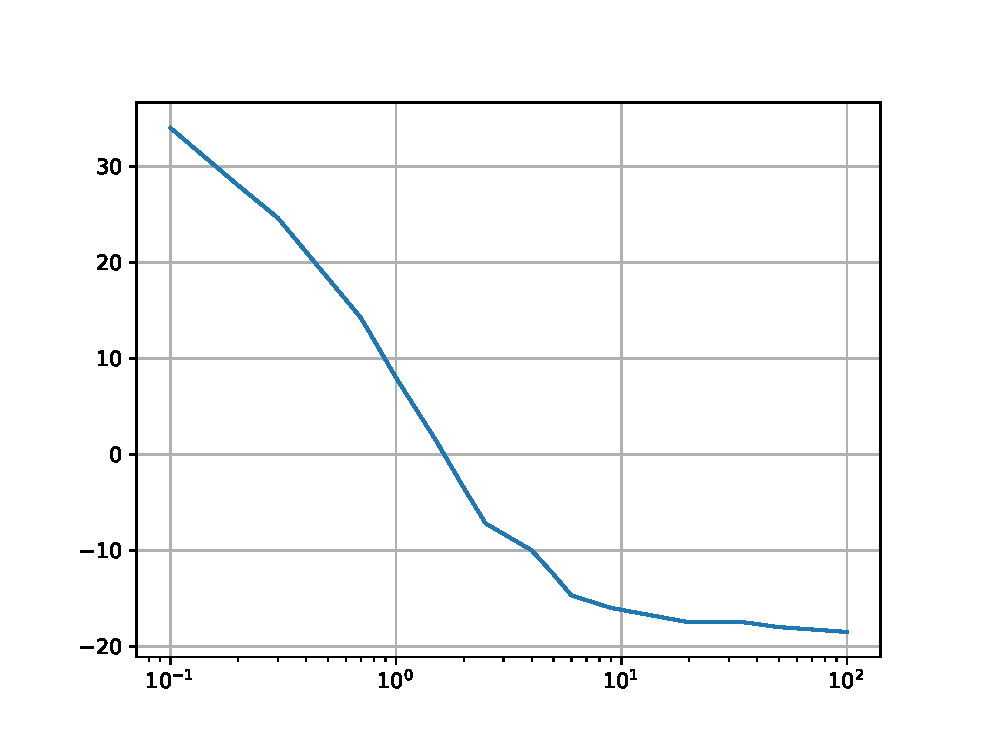
\includegraphics[width=\columnwidth]{./figs/ee18btech11006/ee18btech11006_1.eps}
\caption{1}
\label{fig:ee18btech11006_1}
\end{figure}
Consider the Transfer function
\begin{align}
H(s) &= \frac{k\brak{s+z_{1}}\brak{s+z_{2}}}{\brak{s+p_{1}}\brak{s+p_{2}}} 
\end{align}
Let's draw the magnitude bode plot.
\begin{multline}
20log_{10}|H(s)| = 20log_{10}|s+z_{1}|+20log_{10}|s+z_{2}|\\
-20log_{10}|s+p_{1}|-20log_{10}|s+p_{2}|\\
+20log_{10}k
\end{multline}

Now, for the given set of points finding slopes corresponding to every two points and identifying the points at which the slope change occurs by 20dB would give us the poles and zeros respectively.
The slope initially is-20dB/decade i.e. pole at 0.1 
We can observe that the slope decreases approximately by 20dB/dec at the point 0.7 and increases further by 20dB/dec at 2.5 and 6 giving a slope of almost 0 later on. 
\begin{align}
Poles&= 0.1,0.7\\
Zeros&= 2.5,6
\end{align}
Lets plot the magnitude bode plot considering these poles and zeros.
The following code generates the plot for the transfer function
\begin{align}
H(s) &= \frac{\brak{s+2.5}\brak{s+6}}{\brak{s+0.1}\brak{s+0.7}}
\end{align}
\begin{lstlisting}
codes/ee18btech11006/ee18btech11006_2.py
\end{lstlisting}
\begin{figure}[!ht]
\centering
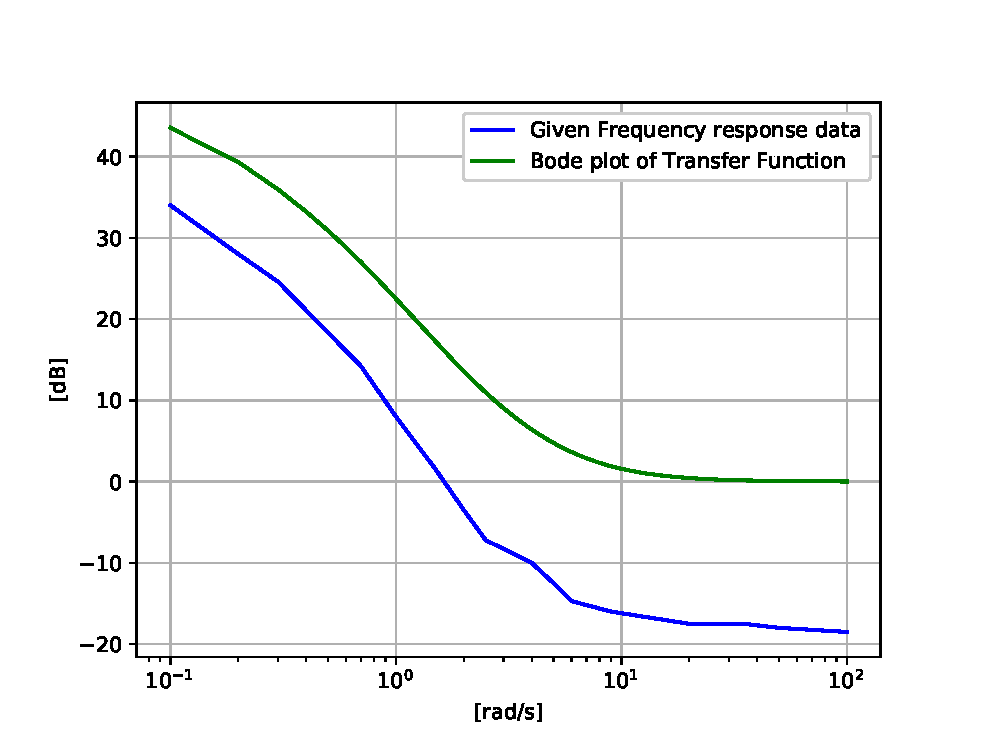
\includegraphics[width=\columnwidth]{./figs/ee18btech11006/ee18btech11006_2.eps}
\caption{2}
\label{fig:ee18btech11006_2}
\end{figure}
Now the gain,
\begin{align}
K=\frac{H\brak{\omega}\brak{given}}{H\brak{\omega}\brak{calculated}} 
\end{align}
This value would vary for different frequencies.
Considering the average value , K= 0.1778. 
The following code generates the plot for the transfer function
\begin{align}
H(s) &= \frac{0.1778\brak{s+2.5}\brak{s+6}}{\brak{s+0.1}\brak{s+0.7}} 
\end{align}
\begin{lstlisting}
codes/ee18btech11006/ee18btech11006_3.py
\end{lstlisting}
\begin{figure}[!ht]
\centering
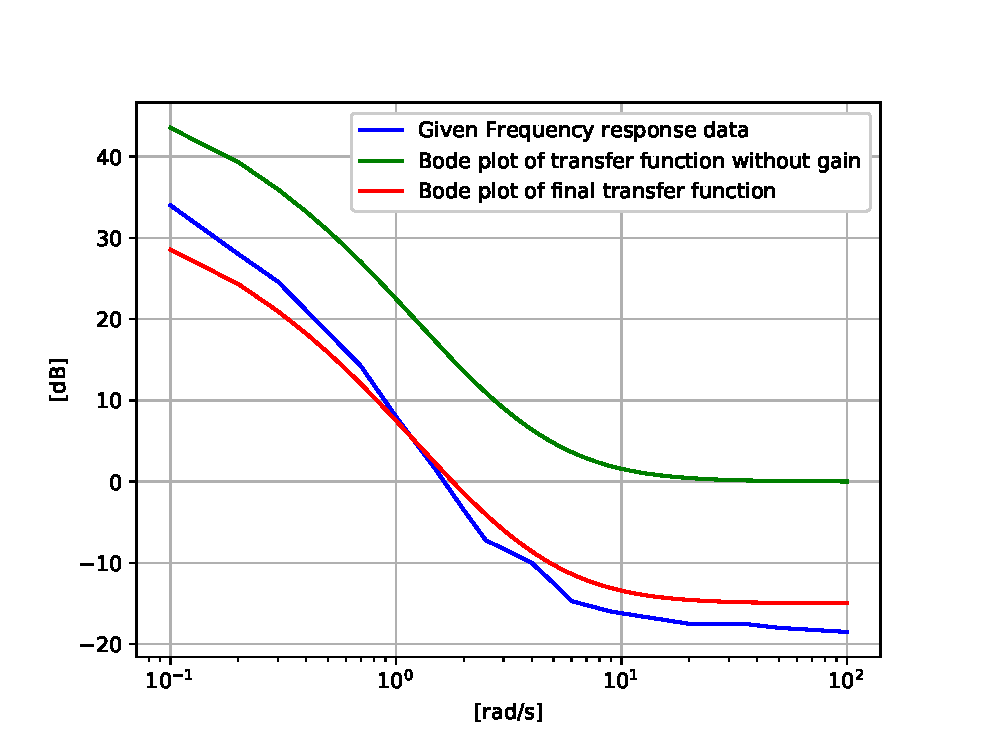
\includegraphics[width=\columnwidth]{./figs/ee18btech11006/ee18btech11006_3.eps}
\caption{3}
\label{fig:ee18btech11006_3}
\end{figure}
Thus, our Transfer function is 
\begin{align}
H(s) &= \frac{0.1778\brak{s+2.5}\brak{s+6}}{\brak{s+0.1}\brak{s+0.7}}  
\end{align}
%\end{enumerate}
